\begin{center}
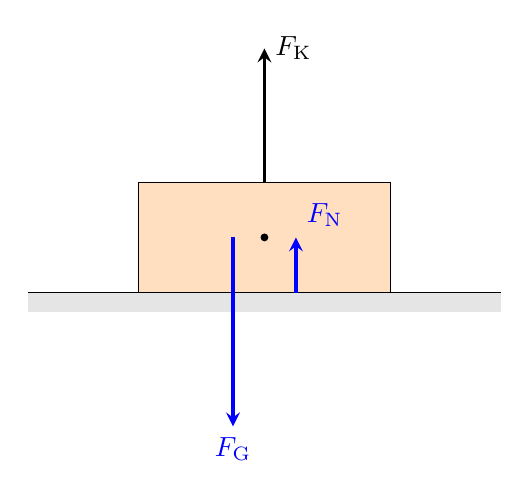
\begin{tikzpicture}[>=stealth]
 \fill[gray!20] (-3,0) rectangle (3,-0.25);
 \draw (-3,0) -- (3,0);
 \draw[fill=orange!25] (-1.6,0) rectangle (1.6,1.4);
 \draw (0,1.4) -- (0,2.2);
 \fill (0,0.7) circle (0.05);
 \draw[->, very thick] (0,1.4) -- ++(0,1.7) node[right] {$F_\mathrm{K}$};
 \draw[->, very thick, blue] (-0.4,0.7) -- ++(0,-2.4) node[below] {$F_\mathrm{G}$};
 \draw[->, very thick, blue] (0.4,0) -- ++(0,0.7) node[anchor=south west] {$F_\mathrm{N}$};
\end{tikzpicture}
\end{center}

Der Container bleibt am Boden in Ruhe, die Kräfte auf ihn sind im Gleichgewicht. Kranseil und Boden tragen zusammen die Gewichtskraft:
\begin{align}
 F_\mathrm{N} + F_\mathrm{K} &= F_\mathrm{G} = m\,g = \FGe
\end{align}
Damit ist die Normalkraft
\begin{align}
 F_\mathrm{N} &= \FNoF \\
   &= \mCo\cdot\gE - \FKr \\
   &= \FNo \approx \result{\FNoP{3}{2}}
\end{align}
